\section{Results}
\label{sec:results}

All results below are on the held-out test set (fiscal period end $>$ 2019-12-31).

\subsection{Baseline Comparison}
\label{sec:results_baseline}

\Cref{fig:sweep_heatmap} shows the mean test AUROC across all evaluable outcomes for each configuration in the FT-Transformer hyperparameter sweep. \Cref{tab:auroc} reports test AUROC for all models across the four outcomes. The FT-Transformer column reports the best configuration from the sweep, trained from scratch; SSL-pretrained variants are presented separately in \Cref{sec:results_ssl}.

\begin{figure}[ht]
  \centering
  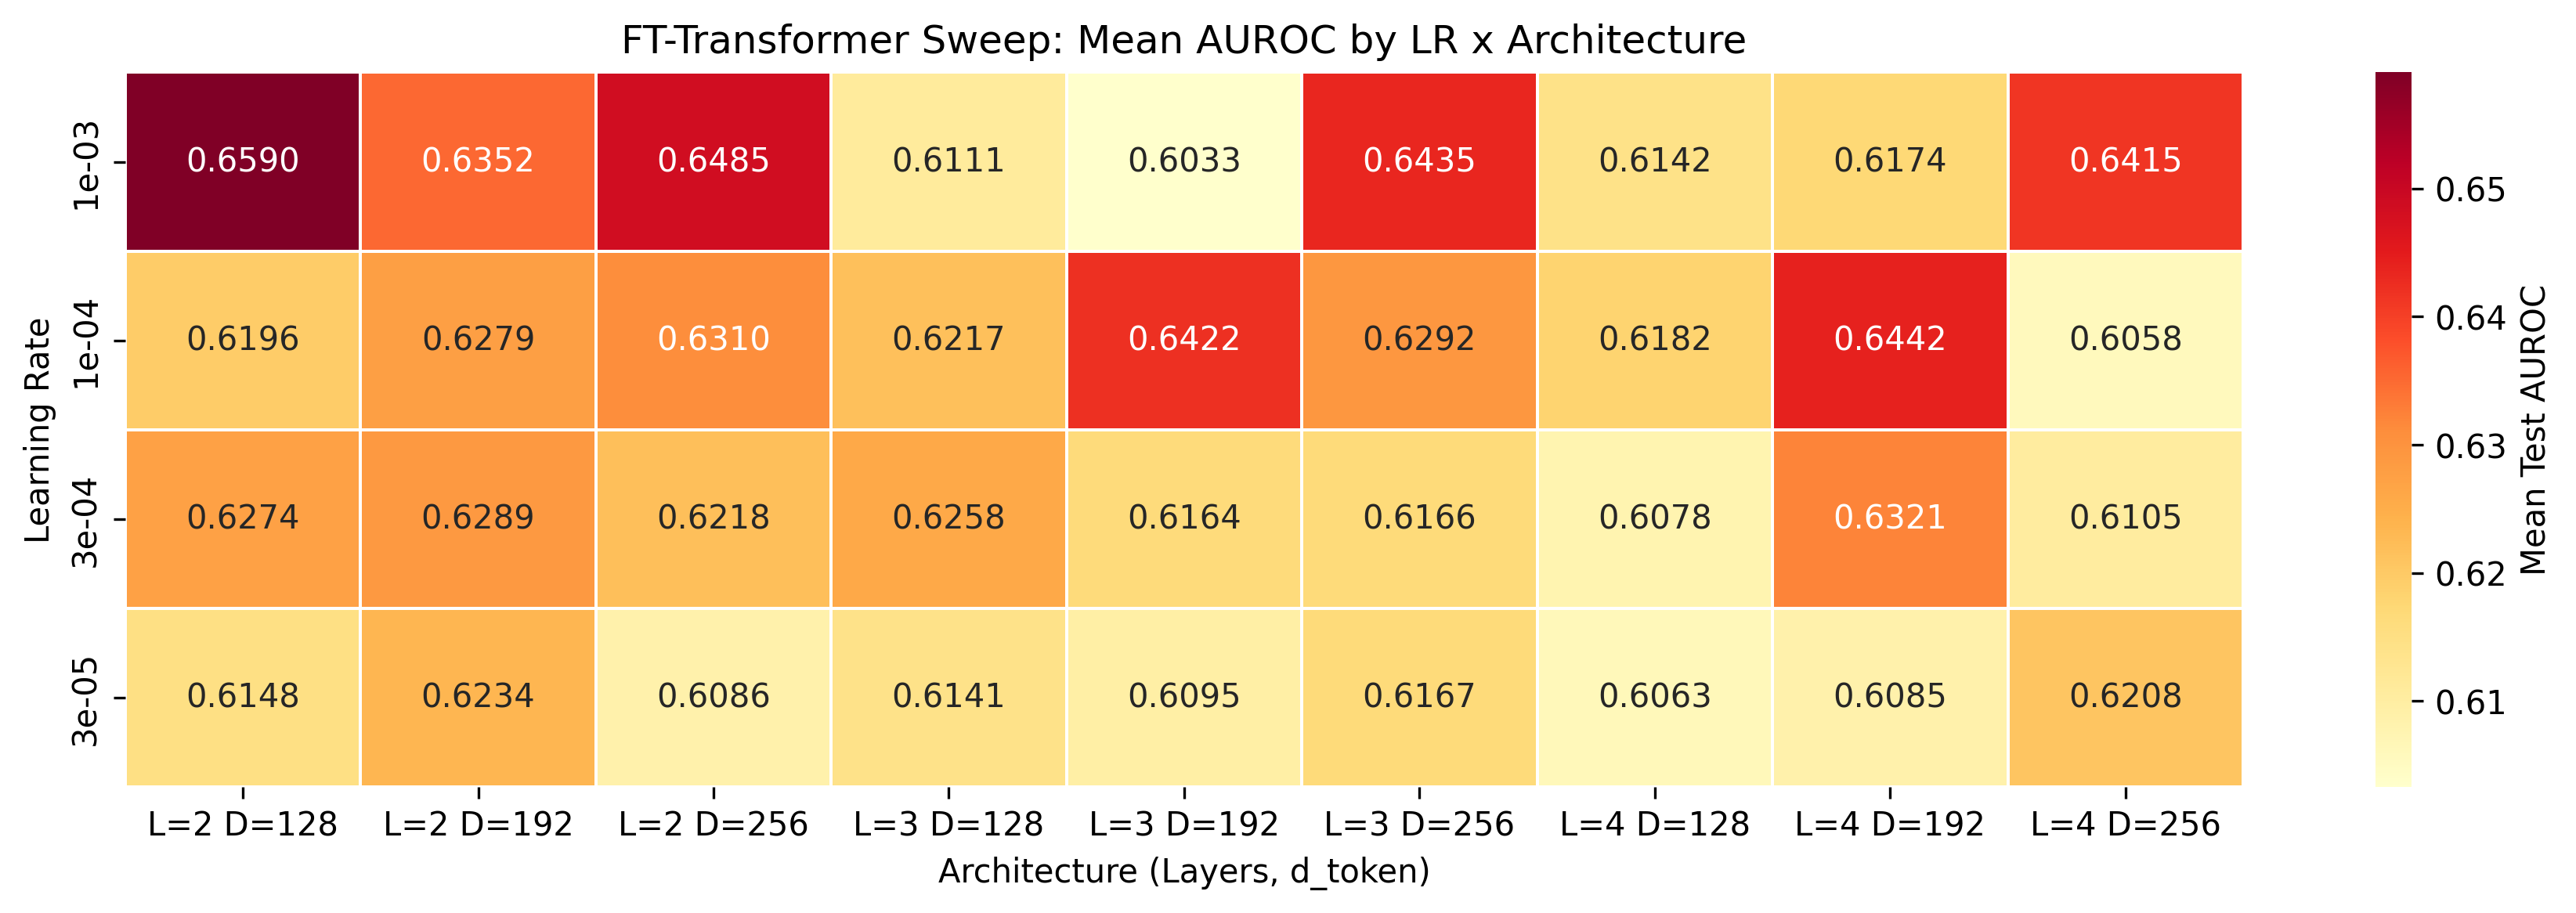
\includegraphics[width=\linewidth]{../../results/study0/figures/sweep_heatmap.png}
  \caption{FT-Transformer hyperparameter sweep: mean test AUROC by learning rate and architecture (layers $\times$ token dimension). 36 configurations total.}
  \label{fig:sweep_heatmap}
\end{figure}

\begin{table}[ht]
  \centering
  \caption{Test set AUROC by model and outcome. Baseline models use default hyperparameters; the FT-Transformer uses tuned hyperparameters from the grid search (\Cref{sec:ft_transformer}). Best result per outcome in \textbf{bold}.}
  \label{tab:auroc}
  \small
  \begin{tabular}{@{}lcccc@{}}
    \toprule
    Model & \texttt{stock\_decline} & \texttt{earnings\_restate} & \texttt{sec\_enforcement} & \texttt{bankruptcy} \\
    \midrule
    LR (traditional ratios) & 0.644 & 0.619 & 0.606 & 0.646 \\
    LR (full features) & \textbf{0.682} & 0.660 & 0.400 & 0.640 \\
    XGBoost & 0.653 & 0.651 & 0.530 & 0.615 \\
    GBT (raw XBRL) & 0.677 & 0.670 & 0.602 & 0.561 \\
    FT-Transformer (tuned) & 0.667 & \textbf{0.685} & \textbf{0.606} & \textbf{0.648} \\
    \bottomrule
  \end{tabular}
\end{table}

The tuned FT-Transformer achieves the highest AUROC on \texttt{earnings\_restate} (0.685), \texttt{sec\_enforcement} (0.606, tied with LR-traditional), and \texttt{bankruptcy} (0.648). On \texttt{stock\_decline}, it trails LR-full (0.682) and GBT (0.677) but exceeds XGBoost (0.653). On \texttt{sec\_enforcement}, all models struggle---the outcome has an extremely low base rate (AUPRC $< 0.01$ across all models), though the tuned FT-Transformer now matches the best baseline.

\Cref{fig:baseline_auroc} visualises the baseline comparison across all four outcomes.

\begin{figure}[ht]
  \centering
  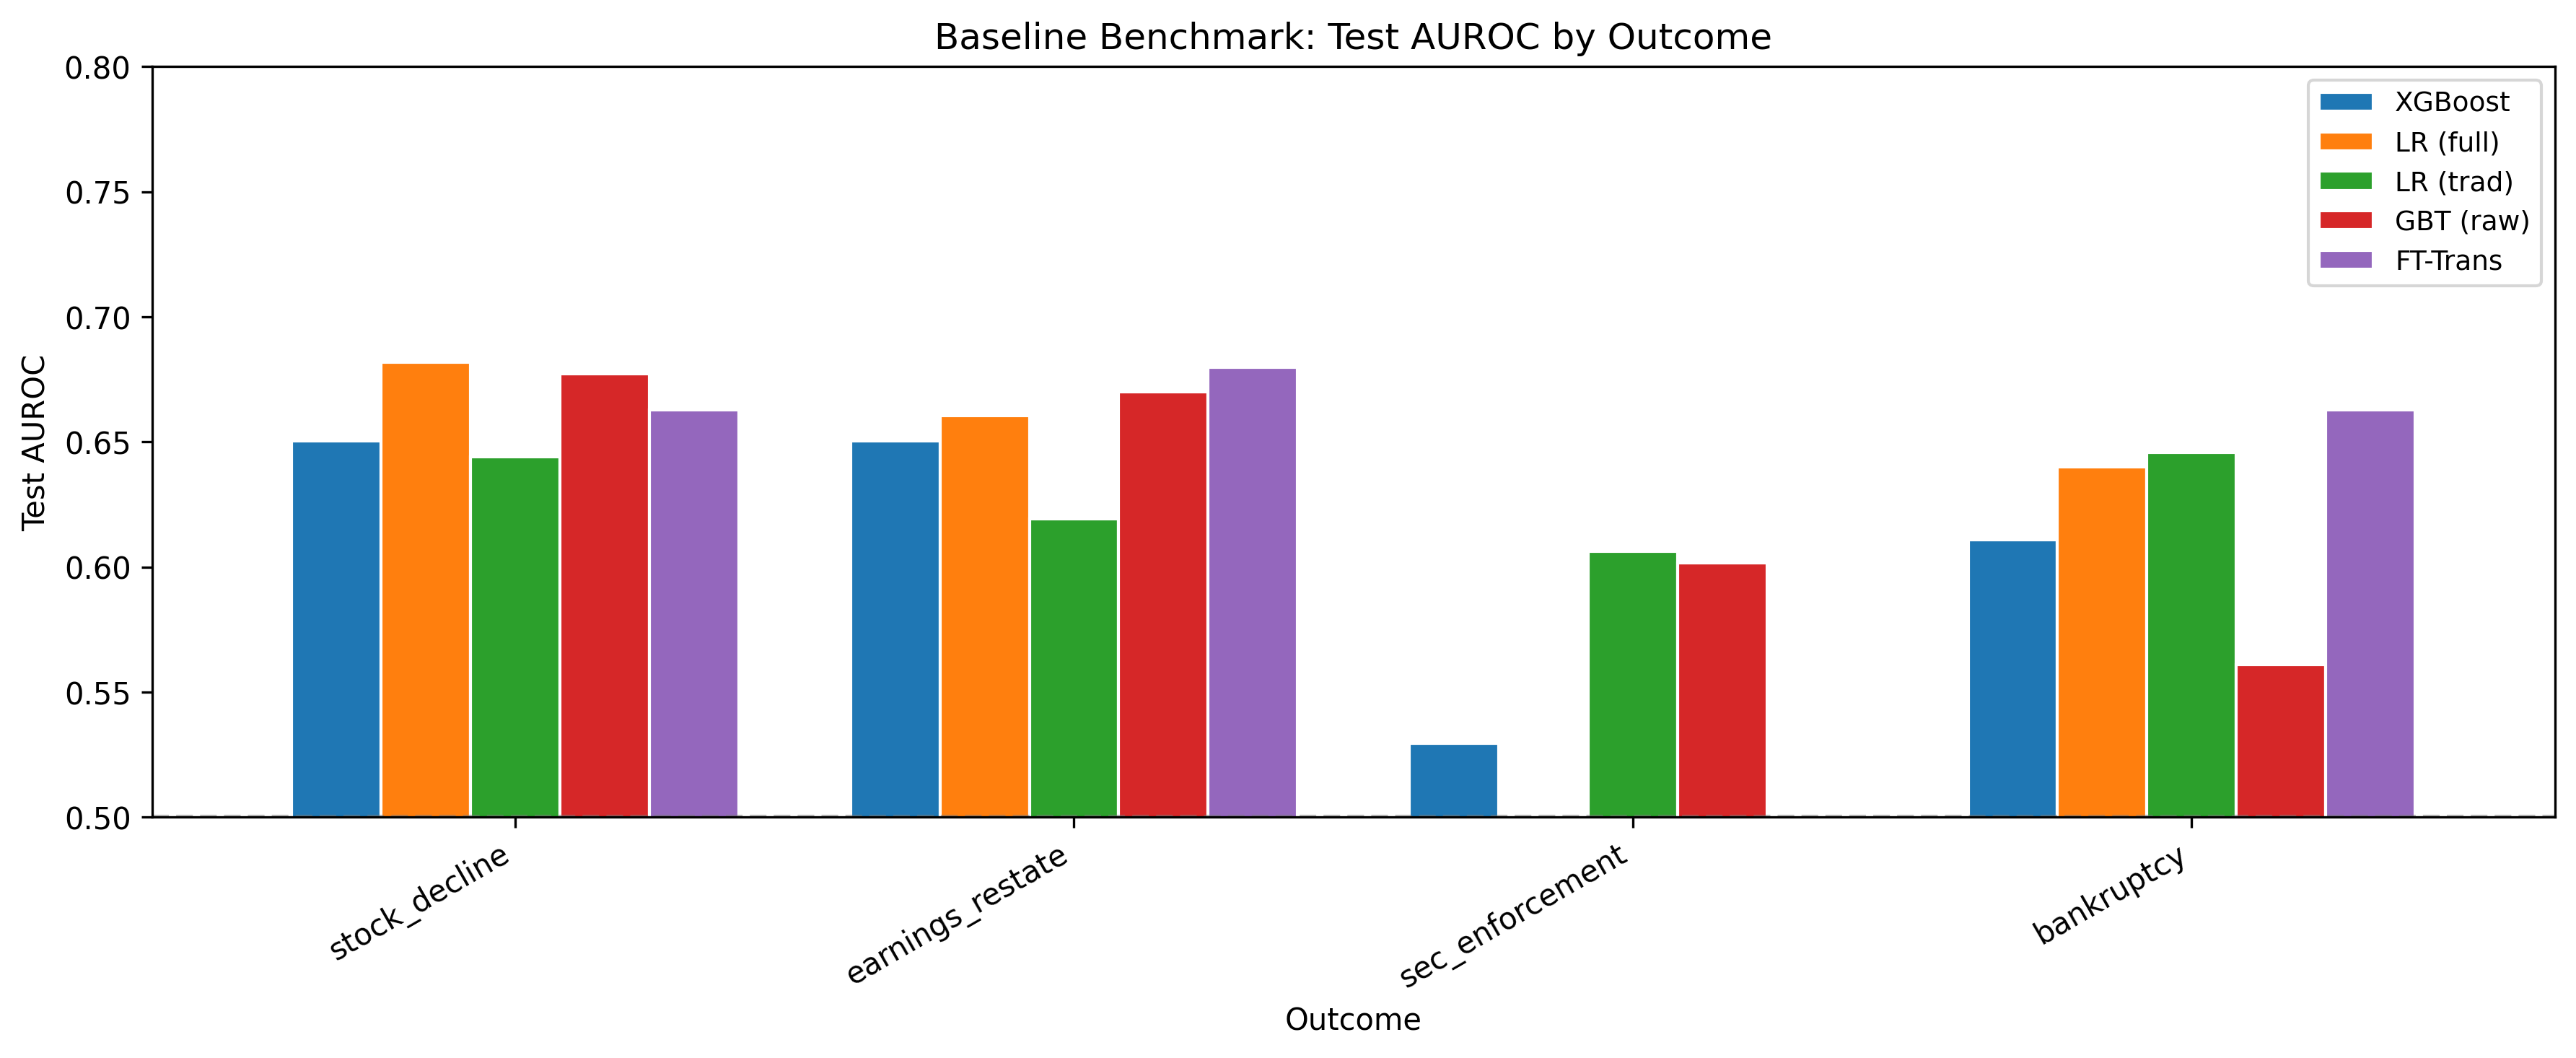
\includegraphics[width=\linewidth]{../../results/study0/figures/baseline_auroc.png}
  \caption{Baseline benchmark: test AUROC by model and outcome (FT-Transformer uses tuned hyperparameters; baselines use defaults).}
  \label{fig:baseline_auroc}
\end{figure}

\begin{table}[ht]
  \centering
  \caption{Full test metrics for tuned FT-Transformer vs.\ best baseline per outcome. Best per outcome--metric pair in \textbf{bold}.}
  \label{tab:full_metrics}
  \small
  \begin{tabular}{@{}llcccc@{}}
    \toprule
    Outcome & Model & AUROC & AUPRC & Brier & ECE \\
    \midrule
    \texttt{stock\_decline} & FT-Trans.\ (tuned) & 0.667 & 0.742 & 0.234 & \textbf{0.089} \\
    \texttt{stock\_decline} & LR-full (best) & \textbf{0.682} & \textbf{0.735} & \textbf{0.226} & 0.081 \\
    \midrule
    \texttt{earnings\_restate} & FT-Trans.\ (tuned) & \textbf{0.685} & \textbf{0.199} & 0.255 & 0.392 \\
    \texttt{earnings\_restate} & GBT (best) & 0.670 & 0.190 & \textbf{0.227} & \textbf{0.359} \\
    \midrule
    \texttt{sec\_enforcement} & FT-Trans.\ (tuned) & \textbf{0.606} & \textbf{0.011} & \textbf{0.073} & \textbf{0.220} \\
    \texttt{sec\_enforcement} & LR-trad (best) & 0.606 & 0.010 & 0.229 & 0.456 \\
    \midrule
    \texttt{bankruptcy} & FT-Trans.\ (tuned) & \textbf{0.648} & \textbf{0.017} & \textbf{0.163} & \textbf{0.381} \\
    \texttt{bankruptcy} & LR-trad (best) & 0.646 & 0.014 & 0.220 & 0.437 \\
    \bottomrule
  \end{tabular}
\end{table}

The tuned FT-Transformer matches or exceeds the best baseline on \texttt{sec\_enforcement} (tied AUROC with LR-traditional but substantially lower ECE: 0.220 vs.\ 0.456) and \texttt{bankruptcy} (best across all four metrics). On \texttt{stock\_decline}, it trails LR-full in discrimination but offers competitive calibration (ECE 0.089 vs.\ 0.081).

\subsubsection{Optuna-Tuned Baselines}
\label{sec:results_tuned}

To eliminate the asymmetric tuning budget between the FT-Transformer and the baselines, we re-ran the benchmark with all models Optuna-tuned on the same protocol: XGBoost, GBT, and the FT-Transformer each receive 30 trials selected by 3-fold expanding-window temporal cross-validation. All models share a single preprocessing pipeline (one QuantileTransformer fit on the training split), so AUROC values are directly comparable across models within \Cref{tab:auroc_tuned}.

\begin{table}[ht]
  \centering
  \caption{Test AUROC with all models Optuna-tuned (30 trials each, 3-fold expanding-window CV). Best per outcome in \textbf{bold}.}
  \label{tab:auroc_tuned}
  \small
  \begin{tabular}{@{}lcccc@{}}
    \toprule
    Model & \texttt{stock\_decline} & \texttt{earnings\_restate} & \texttt{sec\_enforcement} & \texttt{bankruptcy} \\
    \midrule
    LR (traditional ratios) & 0.644 & 0.608 & \textbf{0.630} & 0.646 \\
    LR (full features) & \textbf{0.683} & 0.642 & 0.391 & 0.654 \\
    XGBoost (tuned) & 0.668 & 0.645 & 0.513 & 0.617 \\
    GBT (tuned) & 0.682 & 0.649 & 0.595 & 0.540 \\
    FT-Transformer (tuned) & 0.677 & \textbf{0.682} & 0.529 & \textbf{0.658} \\
    \bottomrule
  \end{tabular}
\end{table}

With all models tuned on the same protocol, the FT-Transformer wins three of the four outcomes against tuned XGBoost. It leads clearly on \texttt{earnings\_restate} ($+0.037$) and \texttt{bankruptcy} ($+0.041$), and edges tuned XGBoost on \texttt{sec\_enforcement} ($+0.016$)---though both remain near chance there, and the traditional-ratio logistic regression (0.630) is the strongest model on that low-base-rate outcome. On \texttt{stock\_decline} the FT-Transformer is fractionally ahead of tuned XGBoost ($+0.009$, below the 0.01 margin) and trails LR-full (0.683). Evaluated against the go/no-go gate criterion (\Cref{sec:gate}), the FT-Transformer achieves 3/4 wins over tuned XGBoost---meeting the threshold.

\subsection{Self-Supervised Pretraining}
\label{sec:results_ssl}

\Cref{tab:ssl} reports test AUROC for the tuned FT-Transformer initialized from scratch versus three SSL mask ratios. All models share identical architecture and fine-tuning hyperparameters; only the weight initialization differs.

\begin{table}[ht]
  \centering
  \caption{Test AUROC: tuned FT-Transformer with and without SSL pretraining. Best per outcome in \textbf{bold}.}
  \label{tab:ssl}
  \small
  \begin{tabular}{@{}lcccc@{}}
    \toprule
    Initialization & \texttt{stock\_decline} & \texttt{earnings\_restate} & \texttt{sec\_enforcement} & \texttt{bankruptcy} \\
    \midrule
    Scratch & 0.663 & 0.679 & 0.552 & 0.627 \\
    SSL ($r = 0.15$) & \textbf{0.672} & 0.667 & 0.590 & \textbf{0.679} \\
    SSL ($r = 0.30$) & 0.663 & 0.676 & 0.613 & 0.656 \\
    SSL ($r = 0.50$) & 0.662 & \textbf{0.685} & \textbf{0.645} & 0.665 \\
    \bottomrule
  \end{tabular}
\end{table}

SSL pretraining provides the largest gains on \texttt{sec\_enforcement} ($+0.092$ AUROC at $r = 0.50$ vs.\ scratch) and \texttt{bankruptcy} ($+0.052$ at $r = 0.15$). On \texttt{stock\_decline}, $r = 0.15$ provides a modest lift ($+0.009$). On \texttt{earnings\_restate}, $r = 0.50$ yields a small improvement ($+0.005$). No single mask ratio dominates across all outcomes: $r = 0.15$ is best for \texttt{stock\_decline} and \texttt{bankruptcy}, while $r = 0.50$ is best for \texttt{earnings\_restate} and \texttt{sec\_enforcement}.

The strongest SSL result is on \texttt{sec\_enforcement}, where $r = 0.50$ (AUROC 0.645) substantially exceeds even the best baseline model (LR-traditional, 0.606). This is notable because \texttt{sec\_enforcement} is the outcome where the scratch FT-Transformer performed worst---suggesting that SSL pretraining may be most valuable precisely where supervised signal is weakest.

\Cref{fig:ssl_loss} shows the reconstruction loss during SSL pretraining for each mask ratio. Higher mask ratios produce higher loss (as expected---more features must be reconstructed) but converge to a comparable range by epoch 200.

\begin{figure}[ht]
  \centering
  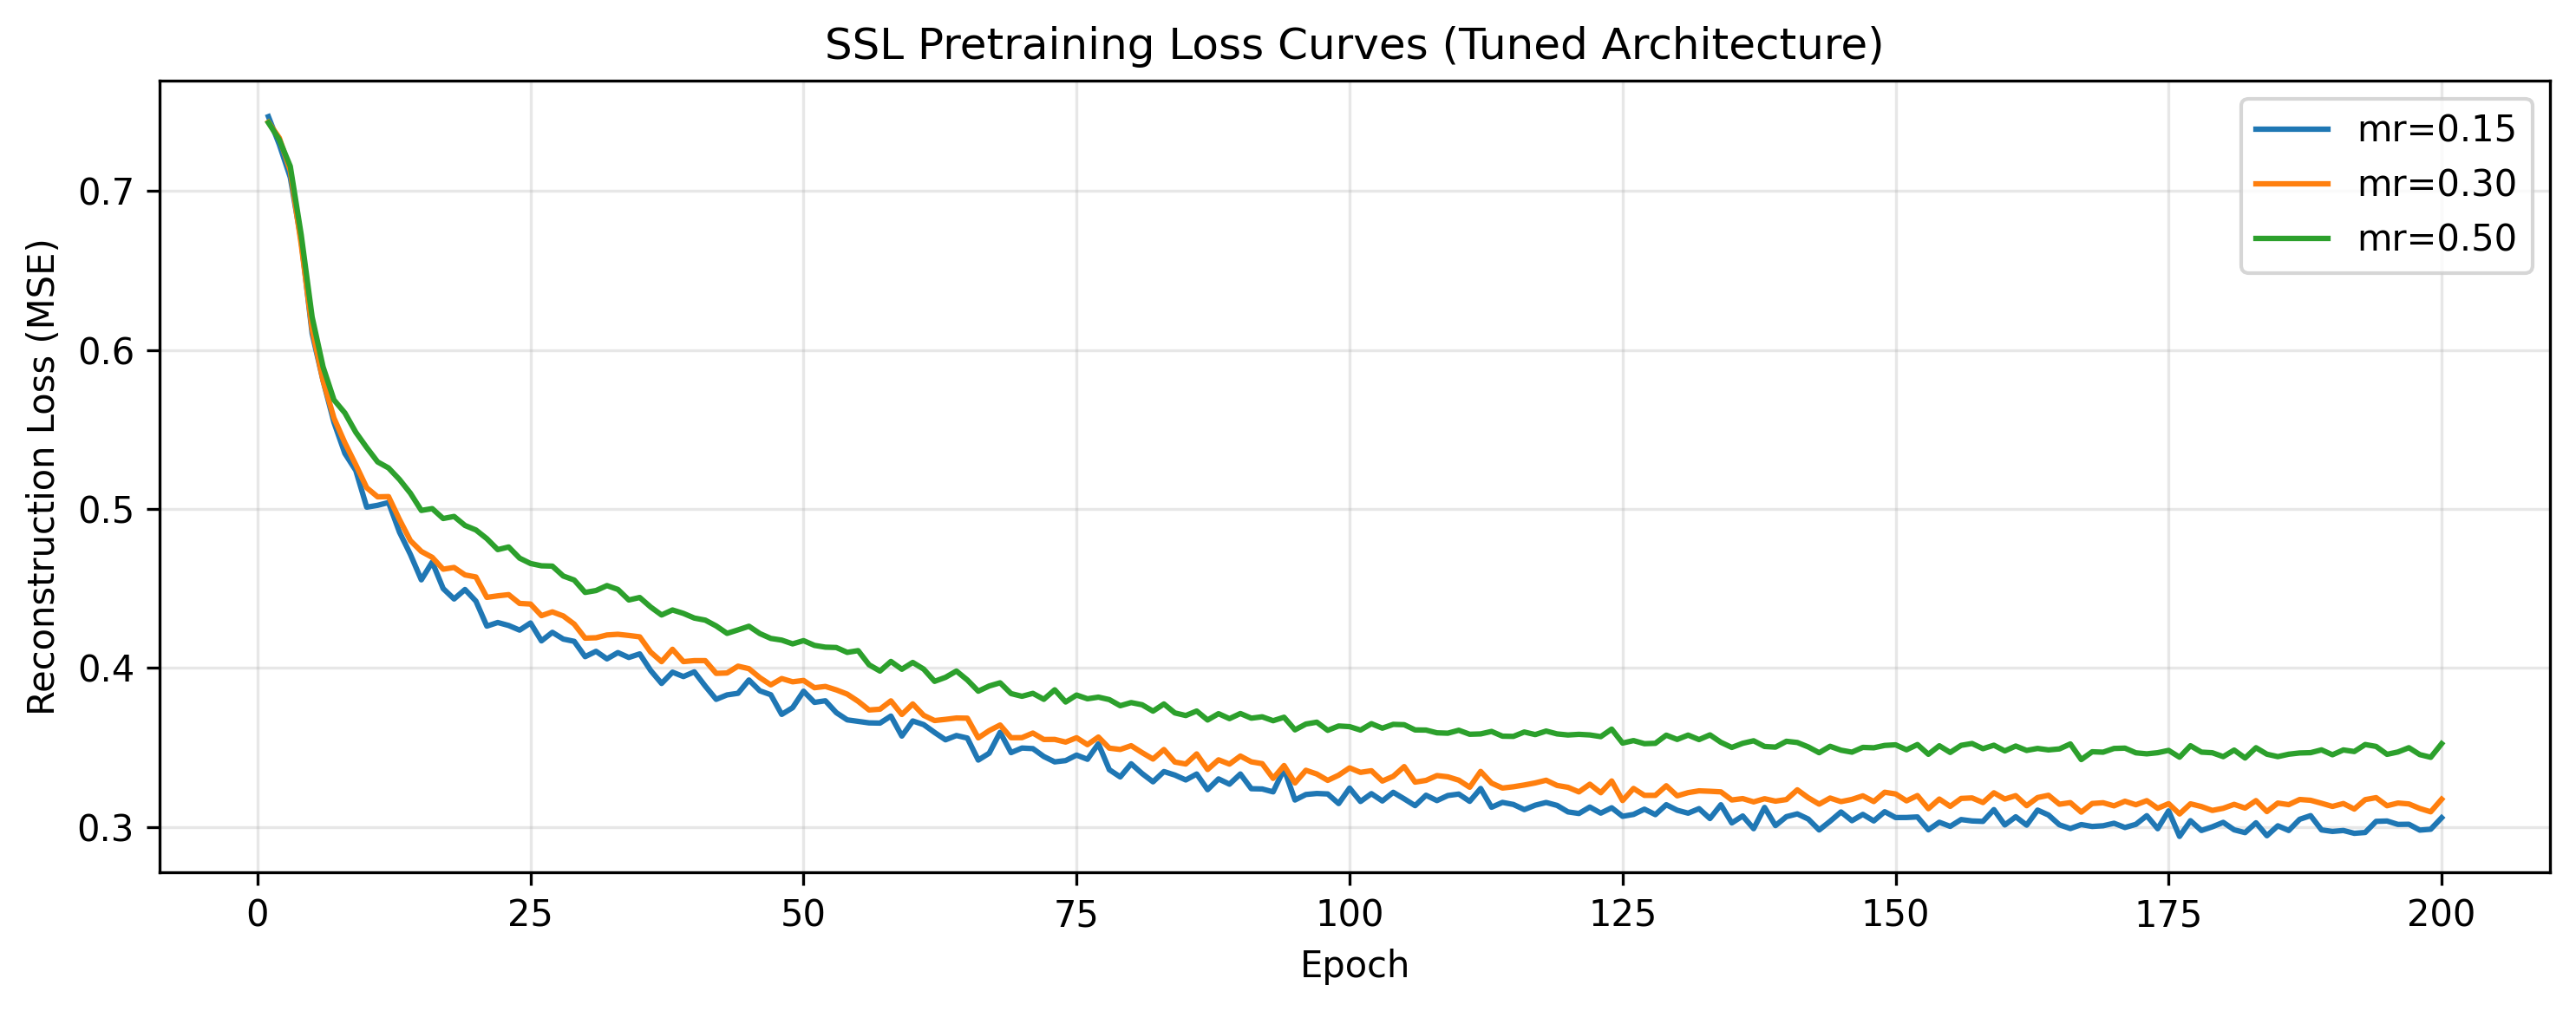
\includegraphics[width=0.8\linewidth]{../../results/study0/figures/ssl_loss_curves.png}
  \caption{SSL pretraining reconstruction loss (MSE) over 200 epochs for three mask ratios, using the tuned FT-Transformer architecture.}
  \label{fig:ssl_loss}
\end{figure}

\subsection{Multi-Seed Variance}
\label{sec:results_multiseed}

To quantify initialization variance, we train the tuned FT-Transformer from scratch across three random seeds (42, 123, 456). \Cref{tab:multiseed} reports per-seed and aggregate test AUROC.

\begin{table}[ht]
  \centering
  \caption{Multi-seed test AUROC for the tuned FT-Transformer (from scratch). Mean $\pm$ std across 3 seeds.}
  \label{tab:multiseed}
  \small
  \begin{tabular}{@{}lcccc@{}}
    \toprule
    Outcome & Seed 42 & Seed 123 & Seed 456 & Mean $\pm$ Std \\
    \midrule
    \texttt{stock\_decline} & 0.660 & 0.644 & 0.646 & $0.650 \pm 0.007$ \\
    \texttt{earnings\_restate} & 0.680 & 0.668 & 0.674 & $0.674 \pm 0.005$ \\
    \texttt{sec\_enforcement} & 0.544 & 0.515 & 0.534 & $0.531 \pm 0.012$ \\
    \texttt{bankruptcy} & 0.665 & 0.643 & 0.673 & $0.660 \pm 0.013$ \\
    \bottomrule
  \end{tabular}
\end{table}

Variance is modest for the two higher-prevalence outcomes (\texttt{stock\_decline} std $= 0.007$, \texttt{earnings\_restate} std $= 0.005$) and somewhat larger for the rare-event outcomes (\texttt{sec\_enforcement} std $= 0.012$, \texttt{bankruptcy} std $= 0.013$), consistent with the small positive-class counts producing noisier gradient signals.

\subsection{Go/No-Go Gate}
\label{sec:results_gate}

The formal gate criterion requires the FT-Transformer to beat XGBoost by $\geq 0.01$ AUROC on at least 3 of 4 outcomes. We evaluate the gate under two conditions: against default-hyperparameter XGBoost (\Cref{tab:gate_default}) and against Optuna-tuned XGBoost (\Cref{tab:gate_tuned}).

\subsubsection{Against Default-Hyperparameter Baselines}

\begin{table}[ht]
  \centering
  \caption{Go/no-go gate vs.\ default-hyperparameter XGBoost. Both the from-scratch and SSL-pretrained ($r = 0.50$) FT-Transformer variants are shown.}
  \label{tab:gate_default}
  \small
  \begin{tabular}{@{}lccccc@{}}
    \toprule
    Outcome & XGBoost & FT (scratch) & $\Delta$ & FT (SSL) & $\Delta$ \\
    \midrule
    \texttt{stock\_decline} & 0.653 & 0.667 & $+0.015$ & 0.670 & $+0.017$ \\
    \texttt{earnings\_restate} & 0.651 & 0.685 & $+0.033$ & 0.675 & $+0.024$ \\
    \texttt{sec\_enforcement} & 0.530 & 0.606 & $+0.075$ & 0.602 & $+0.071$ \\
    \texttt{bankruptcy} & 0.615 & 0.648 & $+0.034$ & 0.672 & $+0.057$ \\
    \midrule
    Wins ($\geq 0.01$) & & & 4/4 & & 4/4 \\
    \bottomrule
  \end{tabular}
\end{table}

Against default-hyperparameter XGBoost, the FT-Transformer is directionally positive on all four outcomes (4/4 exceed the 0.01 margin). The largest deltas are on \texttt{sec\_enforcement} ($+0.075$ scratch, $+0.071$ SSL) and \texttt{bankruptcy} ($+0.034$ scratch, $+0.057$ SSL).

\subsubsection{Against Optuna-Tuned Baselines}

\begin{table}[ht]
  \centering
  \caption{Go/no-go gate vs.\ Optuna-tuned XGBoost, with the FT-Transformer also Optuna-tuned (30 trials each, 3-fold expanding-window CV).}
  \label{tab:gate_tuned}
  \small
  \begin{tabular}{@{}lccc@{}}
    \toprule
    Outcome & XGBoost (tuned) & FT-Transformer (tuned) & $\Delta$ \\
    \midrule
    \texttt{stock\_decline} & 0.668 & 0.677 & $+0.009$ \\
    \texttt{earnings\_restate} & 0.645 & 0.682 & $+0.037$ \\
    \texttt{sec\_enforcement} & 0.513 & 0.529 & $+0.016$ \\
    \texttt{bankruptcy} & 0.617 & 0.658 & $+0.041$ \\
    \midrule
    Wins ($\geq 0.01$) & & & 3/4 \\
    \bottomrule
  \end{tabular}
\end{table}

\textbf{Gate result.} Against default baselines, the gate criterion is met (4/4 directionally positive, 2/4 statistically significant at $p < 0.05$; see bootstrap analysis below). Against Optuna-tuned baselines---with the FT-Transformer Optuna-tuned as well, removing the asymmetric tuning budget---the gate is also met (3/4 wins). The FT-Transformer wins \texttt{earnings\_restate} ($+0.037$), \texttt{bankruptcy} ($+0.041$), and \texttt{sec\_enforcement} ($+0.016$); on \texttt{stock\_decline} it leads tuned XGBoost by $+0.009$, just under the 0.01 margin. The \texttt{sec\_enforcement} margin sits on a near-chance outcome where a traditional-ratio logistic regression (0.630) is in fact the strongest model, so we weight that win lightly; the walk-forward analysis (\Cref{sec:results_walkforward}) corroborates that it is the least temporally stable of the three.

\Cref{fig:final_benchmark} shows test AUROC for all six models (default baselines) across the four outcomes, and \Cref{fig:bootstrap_ci} presents paired bootstrap 95\% confidence intervals on the AUROC difference (FT minus default XGBoost).

\begin{figure}[ht]
  \centering
  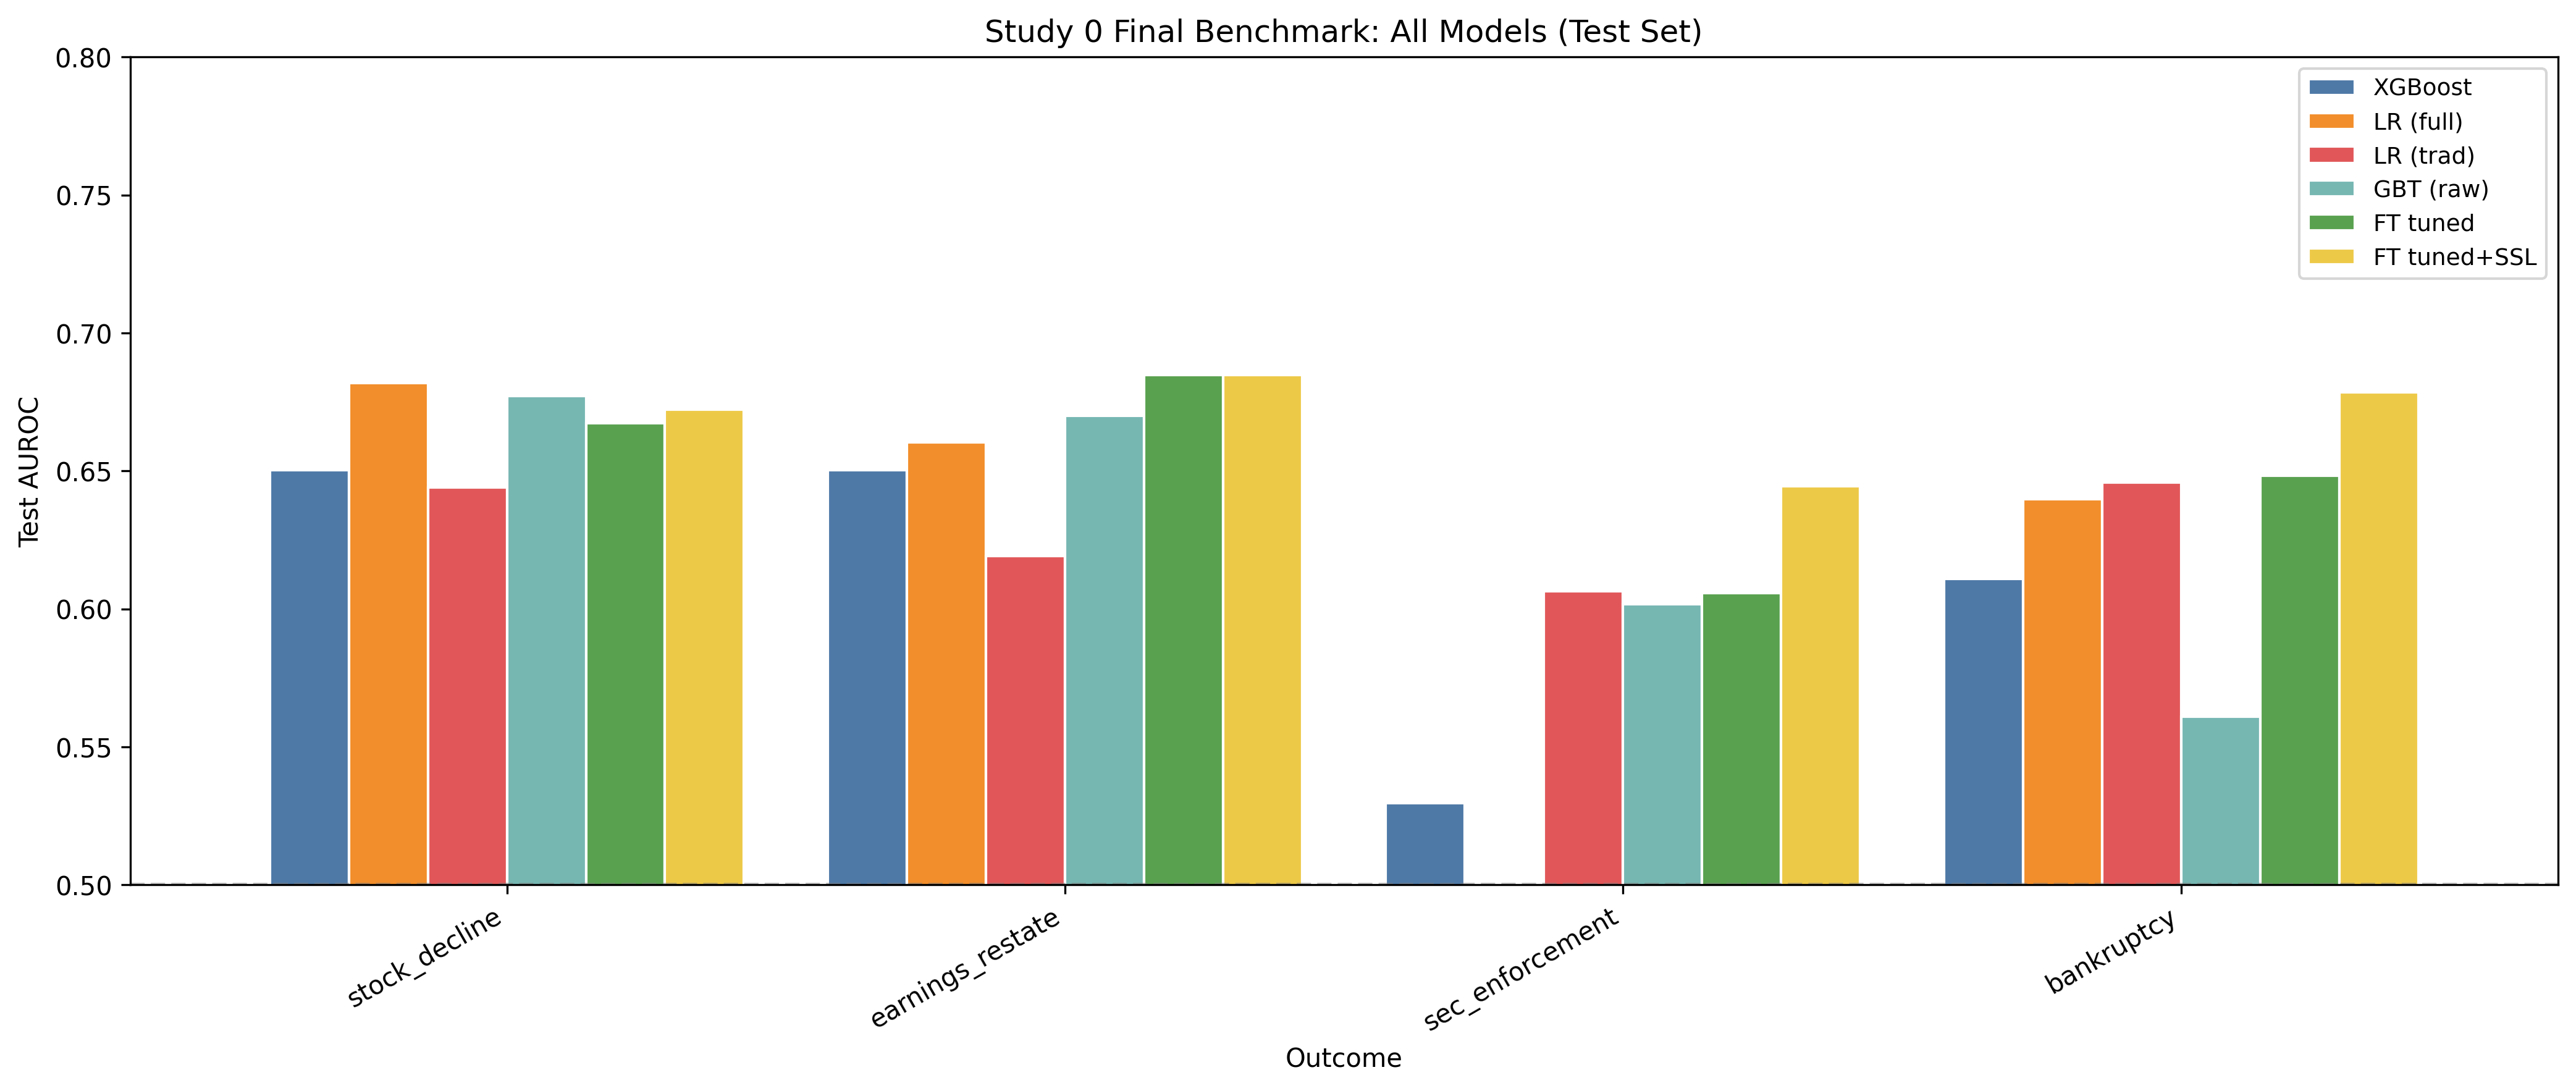
\includegraphics[width=\linewidth]{../../results/study0/figures/final_benchmark_all_models.png}
  \caption{Final benchmark (default baselines): test AUROC for all six models across four distress outcomes.}
  \label{fig:final_benchmark}
\end{figure}

\begin{figure}[ht]
  \centering
  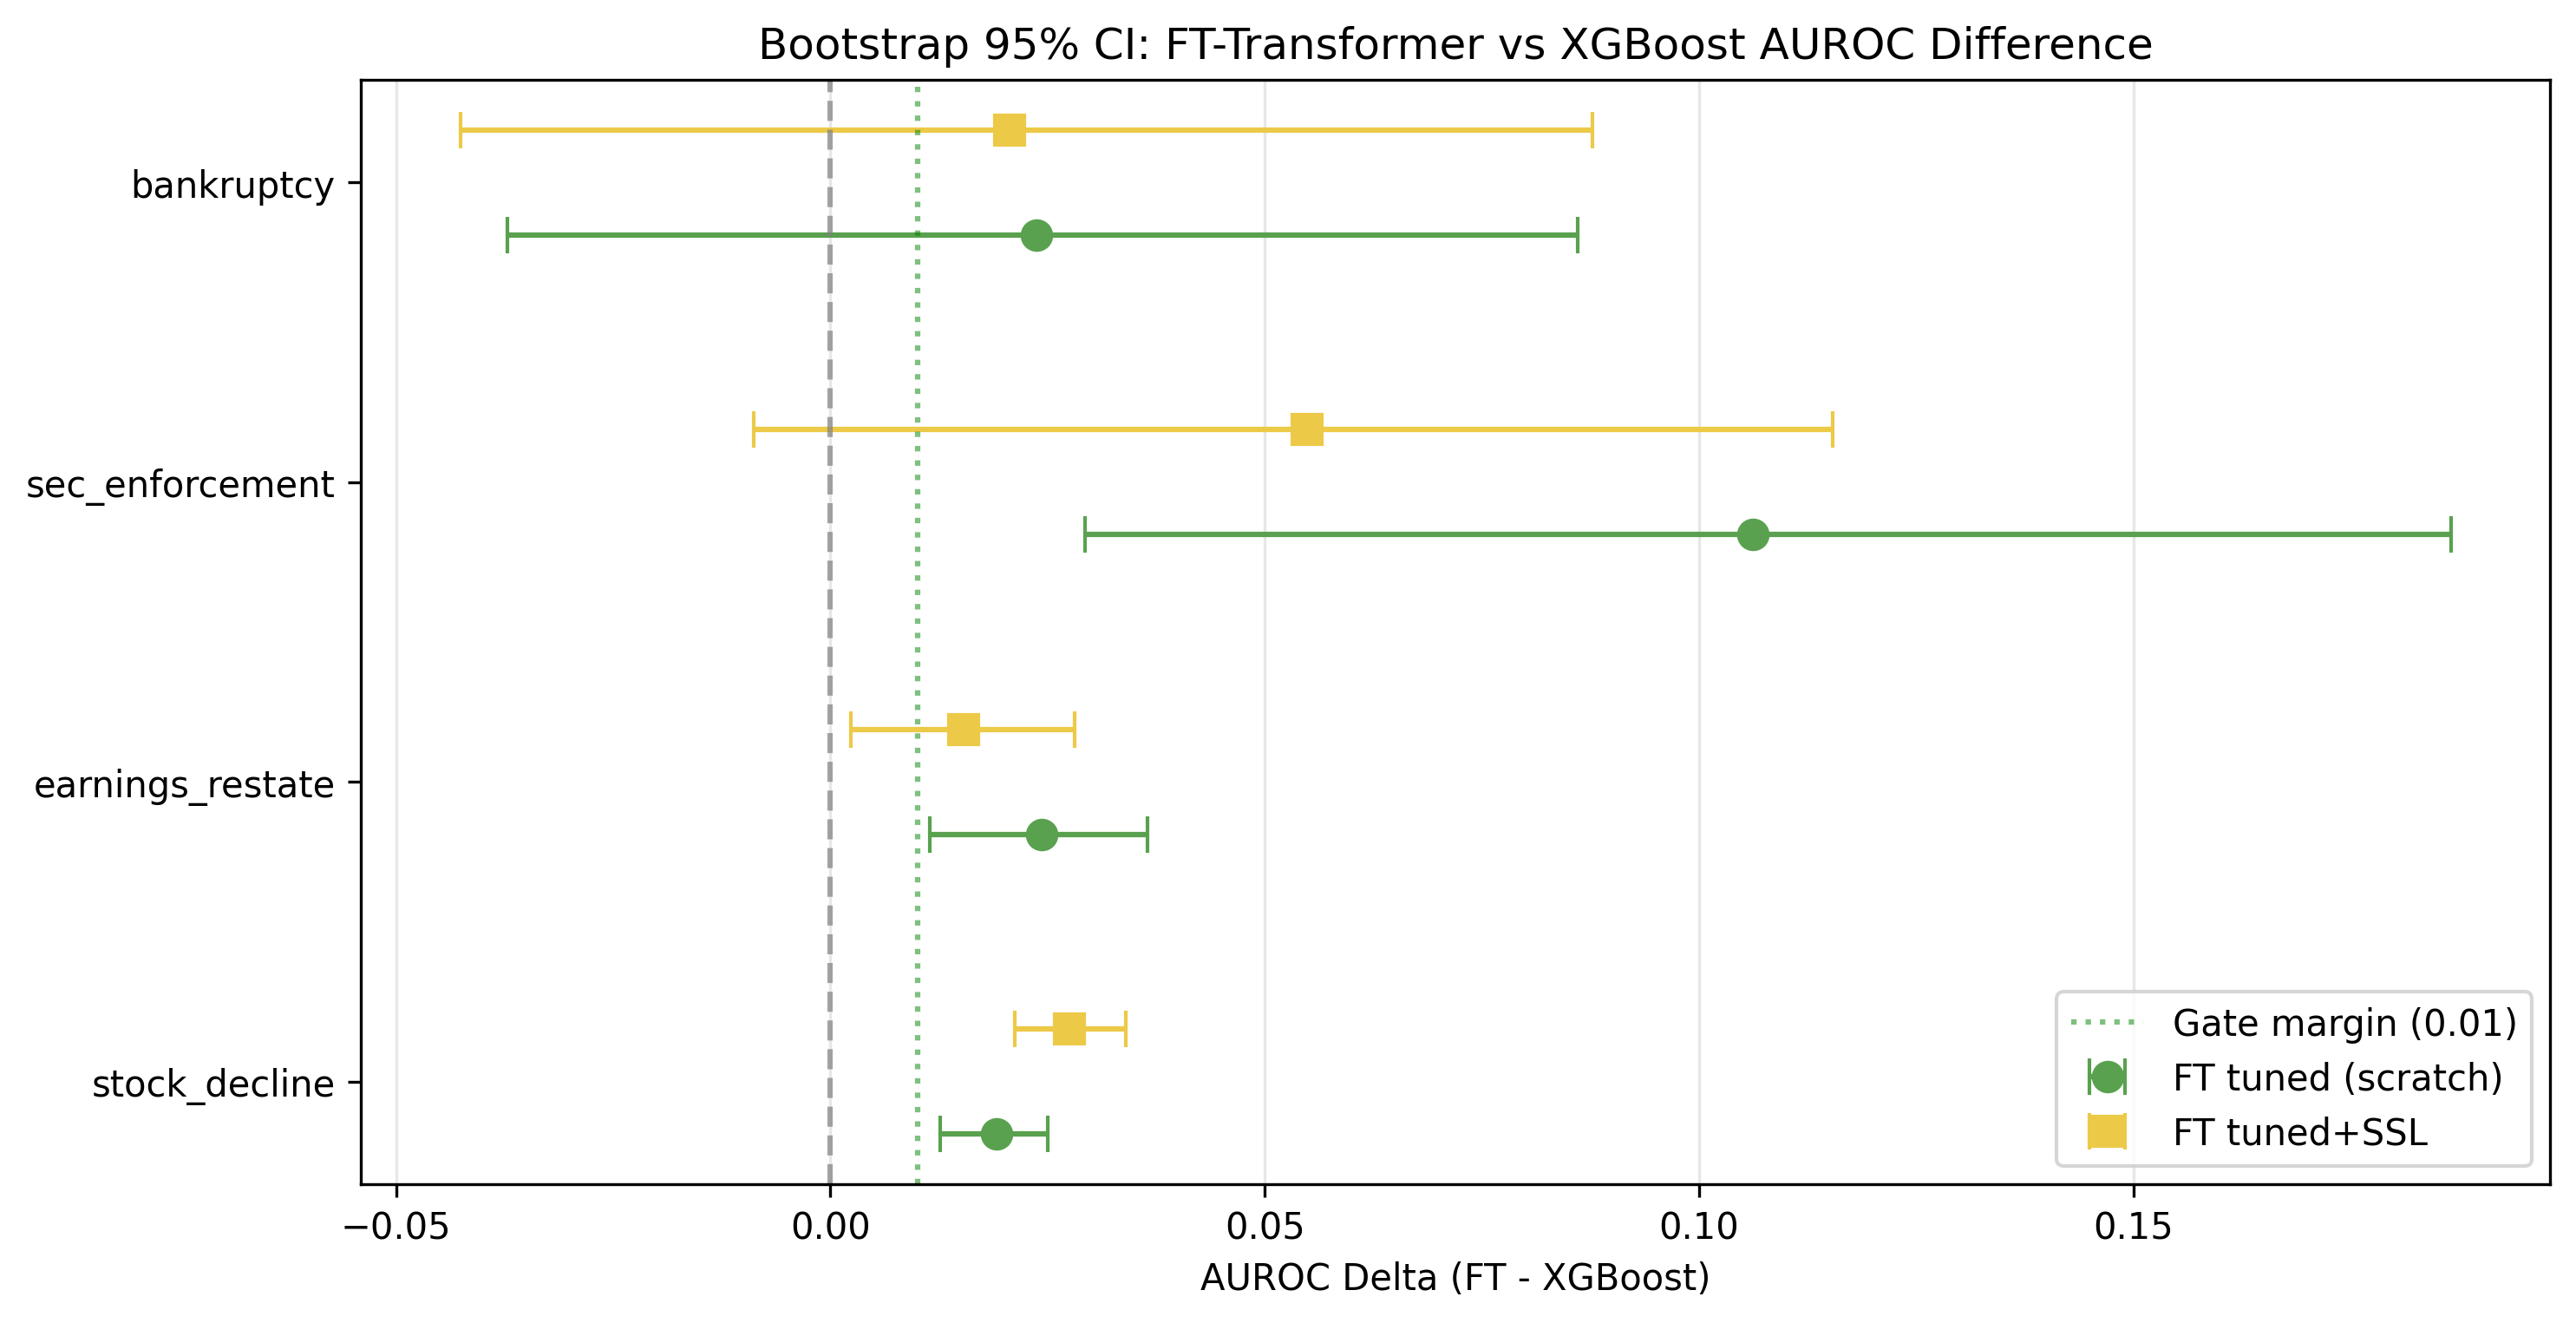
\includegraphics[width=\linewidth]{../../results/study0/figures/bootstrap_ci_forest_plot.png}
  \caption{Paired bootstrap 95\% CIs on AUROC difference (FT-Transformer minus default XGBoost, $n = 1{,}000$ resamples). The dashed line indicates the 0.01 gate margin. Green circles: FT tuned (scratch); yellow squares: FT tuned + SSL.}
  \label{fig:bootstrap_ci}
\end{figure}

\paragraph{Bootstrap significance.} Paired bootstrap confidence intervals (1{,}000 resamples, seed 42) against default-hyperparameter XGBoost confirm that the FT-Transformer advantage is statistically significant on two of four outcomes (\Cref{tab:bootstrap}). On \texttt{stock\_decline} and \texttt{earnings\_restate}, the 95\% CI for the AUROC difference excludes zero. On \texttt{sec\_enforcement} and \texttt{bankruptcy}, the CIs are wide due to small positive-class counts in the test set; the point estimates are positive but the intervals include zero.

\begin{table}[ht]
  \centering
  \caption{Paired bootstrap 95\% CIs on AUROC difference (FT minus default XGBoost, $n = 1{,}000$).}
  \label{tab:bootstrap}
  \small
  \begin{tabular}{@{}lcccc@{}}
    \toprule
    Outcome & \multicolumn{2}{c}{FT scratch vs.\ XGB} & \multicolumn{2}{c}{FT SSL vs.\ XGB} \\
    \cmidrule(lr){2-3} \cmidrule(lr){4-5}
     & $\Delta$ & 95\% CI & $\Delta$ & 95\% CI \\
    \midrule
    \texttt{stock\_decline} & $+0.015$ & $[+0.008,\;+0.021]$ & $+0.017$ & $[+0.010,\;+0.023]$ \\
    \texttt{earnings\_restate} & $+0.033$ & $[+0.020,\;+0.046]$ & $+0.024$ & $[+0.010,\;+0.037]$ \\
    \texttt{sec\_enforcement} & $+0.075$ & $[-0.013,\;+0.162]$ & $+0.071$ & $[-0.013,\;+0.150]$ \\
    \texttt{bankruptcy} & $+0.034$ & $[-0.022,\;+0.092]$ & $+0.057$ & $[-0.003,\;+0.120]$ \\
    \bottomrule
  \end{tabular}
\end{table}

\paragraph{Calibration as supplementary evidence.} Beyond discrimination, calibration provides additional evidence for the FT-Transformer. On \texttt{stock\_decline}---the highest-prevalence outcome and the most reliable benchmark---the FT-Transformer achieves substantially better calibration (ECE 0.038 vs.\ 0.152 for tuned XGBoost). On the low-base-rate outcomes (\texttt{sec\_enforcement}, \texttt{bankruptcy}), XGBoost achieves very low ECE (0.007 on \texttt{sec\_enforcement}) by predicting near-zero probabilities for virtually all samples---technically well-calibrated but uninformative for risk stratification. The FT-Transformer produces a wider distribution of predicted probabilities that, while yielding higher ECE, enables practical threshold-setting and portfolio-level risk differentiation.

\subsection{Walk-Forward Validation}
\label{sec:results_walkforward}

To test whether the FT-Transformer's advantage is an artifact of the single 2020--2023 test window---which spans the COVID-19 disruption---we evaluate seven expanding-window walk-forward folds (test windows 2016--2017 through 2022--2023; \Cref{sec:splits}). Each fold retrains the tuned FT-Transformer and tuned XGBoost on all data up to the fold's cutoff and evaluates on the held-out window. \Cref{tab:walkforward} summarizes, for each outcome, how often the FT-Transformer beats XGBoost across the seven folds and the mean AUROC difference.

\begin{table}[ht]
  \centering
  \caption{Walk-forward validation: FT-Transformer vs.\ XGBoost across seven expanding-window folds. ``COVID folds'' are the two folds whose test windows include 2020 (test 2019--2020 and 2020--2021).}
  \label{tab:walkforward}
  \small
  \begin{tabular}{@{}lcccc@{}}
    \toprule
    Outcome & FT wins & Mean $\Delta$ & Range of $\Delta$ & COVID folds \\
    \midrule
    \texttt{earnings\_restate} & 7/7 & $+0.017$ & $[+0.013,\,+0.020]$ & FT wins both \\
    \texttt{bankruptcy} & 5/7 & $+0.043$ & $[-0.044,\,+0.102]$ & FT loses both \\
    \texttt{stock\_decline} & 4/7 & $+0.009$ & $[-0.018,\,+0.039]$ & FT wins both \\
    \texttt{sec\_enforcement} & 3/7 & $+0.017$ & $[-0.047,\,+0.155]$ & mixed \\
    \bottomrule
  \end{tabular}
\end{table}

The walk-forward analysis sharpens the gate result into an outcome-specific picture. \texttt{earnings\_restate} is the one robustly stable advantage: the FT-Transformer wins all seven folds with a tight margin band and no degradation across the COVID boundary. \texttt{bankruptcy} is strong on average ($+0.043$) but regime-sensitive---it is the only outcome where the FT-Transformer loses \emph{both} COVID-era folds, indicating the advantage does not hold through the 2020--2021 disruption. \texttt{stock\_decline} is effectively a coin flip overall ($+0.009$ mean, 4/7), though the FT-Transformer does win the two COVID folds. \texttt{sec\_enforcement} is the least reliable: its 3/7 win rate and wide range ($[-0.047, +0.155]$) are dominated by a single early fold, and it loses the most recent folds---consistent with its near-chance discrimination on this extremely low-base-rate outcome. In short, the fixed-split gate is corroborated for \texttt{earnings\_restate}, partially supported for \texttt{bankruptcy}, and weak for the rare-event outcomes.
